% System map for the veer-pm-system planning repo.
% Compile: pdflatex system-map.tex  (TeX Live / MacTeX, no exotic packages)
% Companion prose: specs/2026-07-15-system-audit.md
\documentclass[11pt]{article}
\usepackage[margin=1.6cm,landscape,a4paper]{geometry}
\usepackage[T1]{fontenc}
\usepackage{helvet}
\renewcommand{\familydefault}{\sfdefault}
\usepackage{tikz}
\usetikzlibrary{positioning,arrows.meta,shapes.geometric,fit,backgrounds}
\usepackage{booktabs}
\usepackage{xcolor}
\pagestyle{empty}
\setlength{\parindent}{0pt}

\definecolor{mainc}{RGB}{223,235,252}   % main-session work
\definecolor{subc}{RGB}{255,236,210}    % subagent work
\definecolor{extc}{RGB}{222,240,222}    % external service
\definecolor{filec}{RGB}{236,236,236}   % repo file read/write
\definecolor{gatec}{RGB}{250,232,232}   % decision gate

\tikzset{
  box/.style={draw=black!60, rounded corners=2pt, align=center, minimum height=8mm, inner sep=4pt, font=\small},
  main/.style={box, fill=mainc},
  sub/.style={box, fill=subc},
  ext/.style={box, fill=extc},
  file/.style={box, fill=filec},
  gate/.style={draw=black!60, diamond, aspect=2.4, align=center, fill=gatec, inner sep=1pt, font=\small},
  flow/.style={-{Stealth[length=2.5mm]}, thick, black!70},
  opt/.style={flow, dashed},
  lane/.style={draw=black!25, rounded corners=3pt, inner xsep=6pt, inner ysep=15pt},
  lanelabel/.style={font=\footnotesize\bfseries, text=black!60, rotate=90, anchor=south, align=center}
}

\begin{document}

{\Large\bfseries veer-pm-system: system map}\hfill{\small 2026-07-15}

\vspace{2mm}
Legend:\quad
\tikz{\node[main, minimum height=5mm]{main session};}\quad
\tikz{\node[sub, minimum height=5mm]{subagent (cheaper model)};}\quad
\tikz{\node[ext, minimum height=5mm]{external service};}\quad
\tikz{\node[file, minimum height=5mm]{repo file};}\quad
\tikz{\node[gate, minimum height=5mm, aspect=3]{gate};}\quad
dashed = conditional

\newpage
{\large\bfseries 1. Veer's journeys: every entry point and where it leads}

\vspace{1mm}
Every journey passes the same front door and exit. Journeys chain freely in one day: initialize $\to$ tutor $\to$ debrief is one day, three journeys.

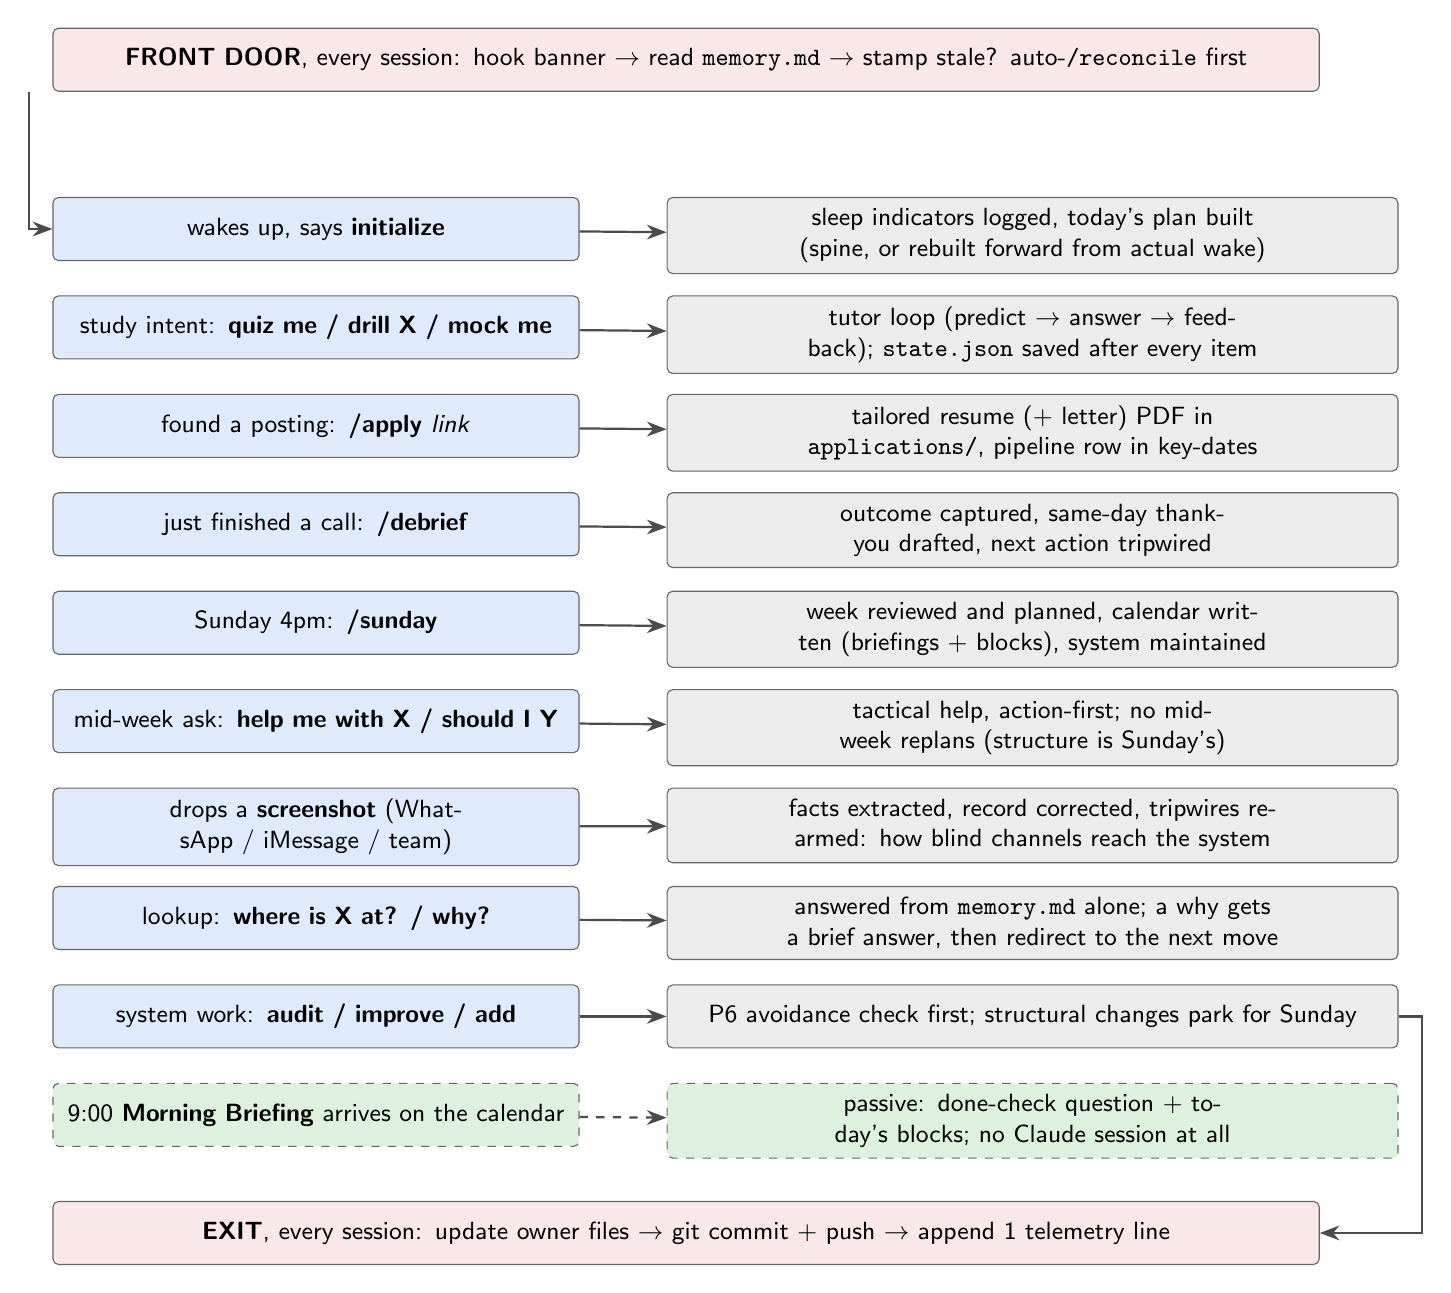
\begin{tikzpicture}
  \node[box, fill=gatec, text width=158mm, anchor=north west] (front) at (0,0.9) {\textbf{FRONT DOOR}, every session: hook banner $\to$ read \texttt{memory.md} $\to$ stamp stale? auto-\texttt{/reconcile} first};

  \newcommand{\jrow}[4]{
    \node[main, text width=64mm, anchor=north west] (e#1) at (0,#2) {#3};
    \node[file, text width=90mm, anchor=north west] (o#1) at (7.8,#2) {#4};
    \draw[flow] (e#1) -- (o#1);
  }
  \jrow{1}{-1.25}{wakes up, says \textbf{initialize}}{sleep indicators logged, today's plan built (spine, or rebuilt forward from actual wake)}
  \jrow{2}{-2.50}{study intent: \textbf{quiz me / drill X / mock me}}{tutor loop (predict $\to$ answer $\to$ feedback); \texttt{state.json} saved after every item}
  \jrow{3}{-3.75}{found a posting: \textbf{/apply} \textit{link}}{tailored resume (+ letter) PDF in \texttt{applications/}, pipeline row in key-dates}
  \jrow{4}{-5.00}{just finished a call: \textbf{/debrief}}{outcome captured, same-day thank-you drafted, next action tripwired}
  \jrow{5}{-6.25}{Sunday 4pm: \textbf{/sunday}}{week reviewed and planned, calendar written (briefings + blocks), system maintained}
  \jrow{6}{-7.50}{mid-week ask: \textbf{help me with X / should I Y}}{tactical help, action-first; no mid-week replans (structure is Sunday's)}
  \jrow{7}{-8.75}{drops a \textbf{screenshot} (WhatsApp / iMessage / team)}{facts extracted, record corrected, tripwires re-armed: how blind channels reach the system}
  \jrow{8}{-10.00}{lookup: \textbf{where is X at? / why?}}{answered from \texttt{memory.md} alone; a why gets a brief answer, then redirect to the next move}
  \jrow{9}{-11.25}{system work: \textbf{audit / improve / add}}{P6 avoidance check first; structural changes park for Sunday}

  \node[ext, text width=64mm, anchor=north west, dashed] (e10) at (0,-12.5) {9:00 \textbf{Morning Briefing} arrives on the calendar};
  \node[ext, text width=90mm, anchor=north west, dashed] (o10) at (7.8,-12.5) {passive: done-check question + today's blocks; no Claude session at all};
  \draw[opt] (e10) -- (o10);

  \node[box, fill=gatec, text width=158mm, anchor=north west] (exit) at (0,-14.0) {\textbf{EXIT}, every session: update owner files $\to$ git commit + push $\to$ append 1 telemetry line};

  \draw[flow] ([xshift=-3mm]front.south west) ++(0,0) |- (e1.west);
  \draw[flow] (o9.east) -- ++(0.3,0) |- (exit.east);
\end{tikzpicture}

\newpage
{\large\bfseries 2. Every session: the lifecycle}

\vspace{4mm}
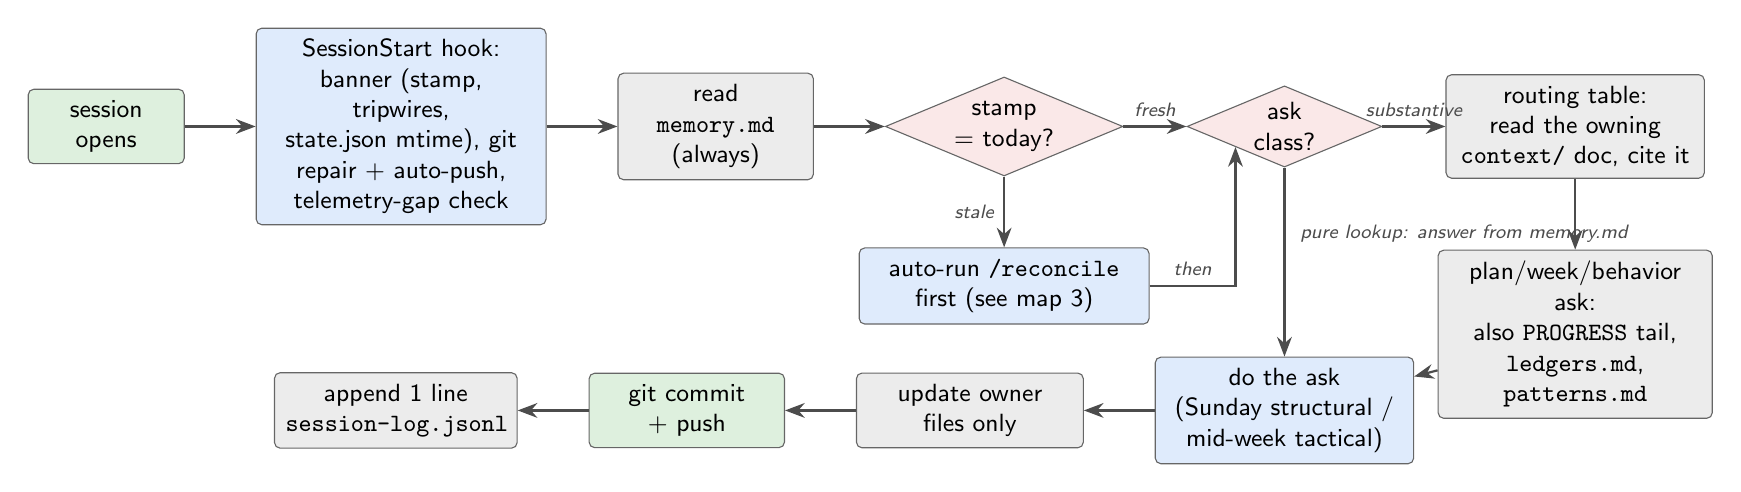
\begin{tikzpicture}[node distance=6mm and 9mm]
  \node[ext, text width=17mm] (open) {session\\opens};
  \node[main, text width=34mm, right=of open] (hook) {SessionStart hook:\\banner (stamp, tripwires,\\state.json mtime), git\\repair + auto-push,\\telemetry-gap check};
  \node[file, text width=22mm, right=of hook] (mem) {read\\\texttt{memory.md}\\(always)};
  \node[gate, right=of mem] (g1) {stamp\\= today?};
  \node[gate, right=8mm of g1] (g2) {ask\\class?};
  \node[file, text width=30mm, right=8mm of g2] (route) {routing table:\\read the owning\\\texttt{context/} doc, cite it};

  \node[main, text width=34mm, below=9mm of g1] (rec) {auto-run \texttt{/reconcile}\\first (see map 3)};
  \node[file, text width=32mm, below=9mm of route] (extra) {plan/week/behavior ask:\\also \texttt{PROGRESS} tail,\\\texttt{ledgers.md}, \texttt{patterns.md}};

  \node[main, text width=30mm, below=24mm of g2] (work) {do the ask\\(Sunday structural /\\mid-week tactical)};
  \node[file, text width=26mm, left=of work] (persist) {update owner\\files only};
  \node[ext, text width=22mm, left=of persist] (commit) {git commit\\+ push};
  \node[file, text width=28mm, left=of commit] (tel) {append 1 line\\\texttt{session-log.jsonl}};

  \draw[flow] (open) -- (hook);
  \draw[flow] (hook) -- (mem);
  \draw[flow] (mem) -- (g1);
  \draw[flow] (g1) -- node[above, font=\scriptsize\itshape]{fresh} (g2);
  \draw[flow] (g1) -- node[left, font=\scriptsize\itshape]{stale} (rec);
  \draw[flow] (rec.east) -| node[near start, above, font=\scriptsize\itshape]{then} (g2.south west);
  \draw[flow] (g2) -- node[above, font=\scriptsize\itshape]{substantive} (route);
  \draw[flow] (g2.south) -- node[right=2pt, font=\scriptsize\itshape, pos=0.35]{pure lookup: answer from memory.md} (work.north);
  \draw[flow] (route) -- (extra);
  \draw[flow] (extra) -- (work);
  \draw[flow] (work) -- (persist);
  \draw[flow] (persist) -- (commit);
  \draw[flow] (commit) -- (tel);
\end{tikzpicture}

\vspace{5mm}
The only fixed context cost every session pays is the hook banner plus \texttt{memory.md} ($\sim$100 lines). Everything else is gated by the ask.

\newpage
{\large\bfseries 3. \texttt{/reconcile}: the one workflow that spawns subagents}

\vspace{4mm}
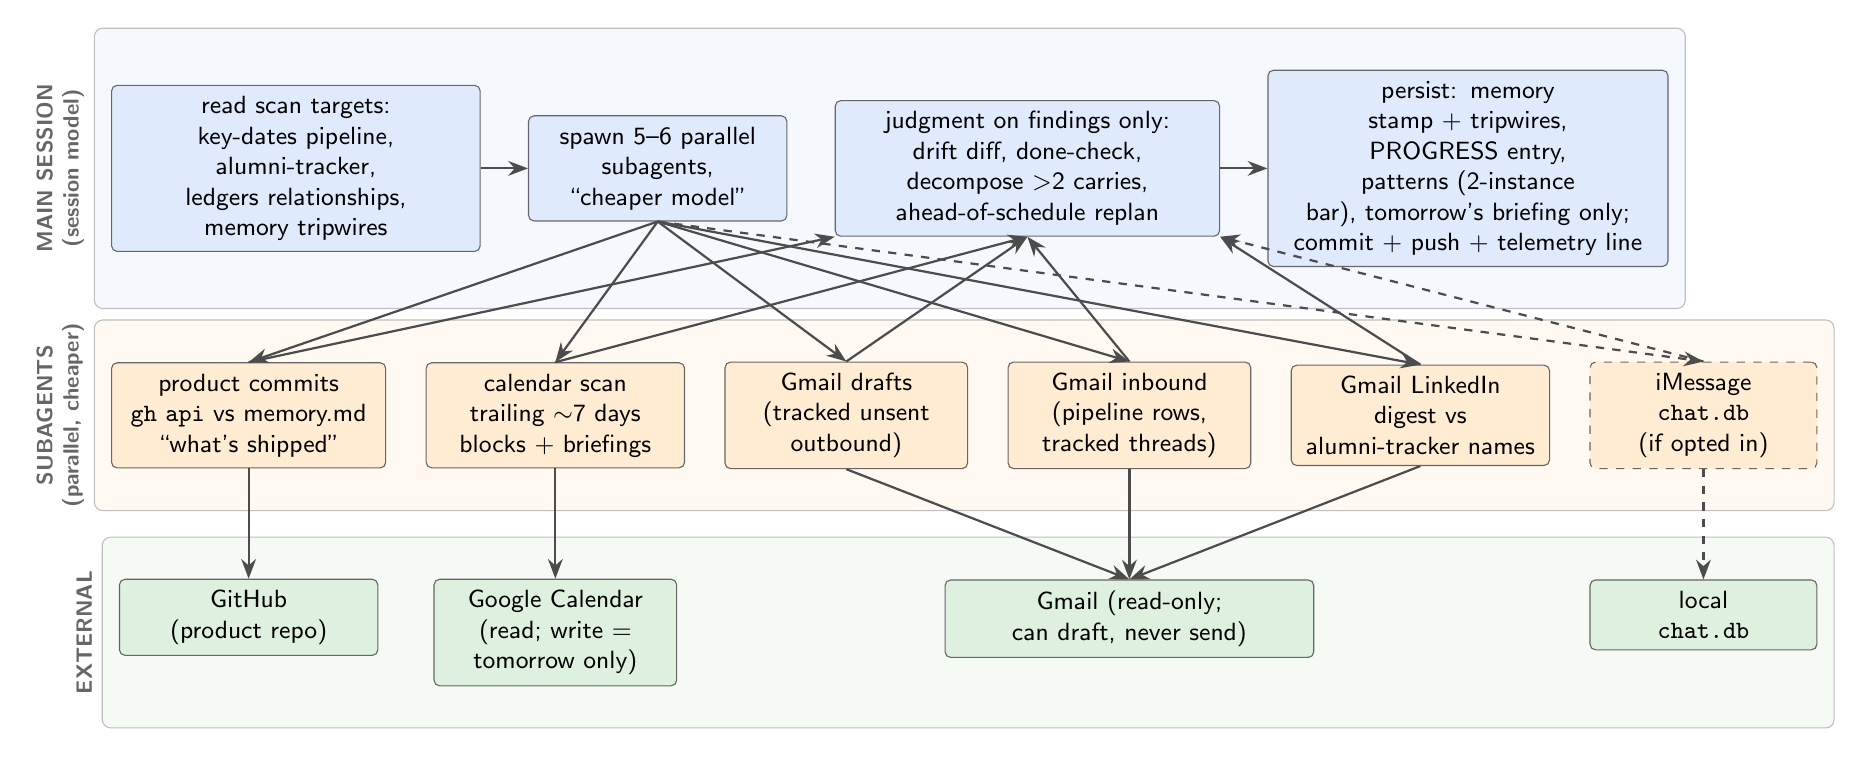
\begin{tikzpicture}[node distance=5mm and 5mm]
  % ---- subagent lane (middle) ----
  \node[sub, text width=32mm] (commits) {product commits\\\texttt{gh api} vs memory.md\\``what's shipped''};
  \node[sub, text width=30mm, right=of commits] (cal) {calendar scan\\trailing $\sim$7 days\\blocks + briefings};
  \node[sub, text width=28mm, right=of cal] (gd) {Gmail drafts\\(tracked unsent\\outbound)};
  \node[sub, text width=28mm, right=of gd] (gi) {Gmail inbound\\(pipeline rows,\\tracked threads)};
  \node[sub, text width=30mm, right=of gi] (gl) {Gmail LinkedIn\\digest vs\\alumni-tracker names};
  \node[sub, text width=26mm, right=of gl, dashed] (im) {iMessage\\\texttt{chat.db}\\(if opted in)};

  % ---- main lane (top) ----
  \node[main, text width=44mm, above=14mm of commits.north west, anchor=south west] (targets) {read scan targets:\\key-dates pipeline, alumni-tracker,\\ledgers relationships, memory tripwires};
  \node[main, text width=30mm, right=6mm of targets] (spawn) {spawn 5--6 parallel\\subagents,\\``cheaper model''};
  \node[main, text width=46mm, right=6mm of spawn] (judge) {judgment on findings only:\\drift diff, done-check,\\decompose $>$2 carries,\\ahead-of-schedule replan};
  \node[main, text width=48mm, right=6mm of judge] (writes) {persist: memory stamp + tripwires,\\PROGRESS entry, patterns (2-instance\\bar), tomorrow's briefing only;\\commit + push + telemetry line};

  % ---- external lane (bottom) ----
  \node[ext, text width=30mm, below=14mm of commits] (gh) {GitHub\\(product repo)};
  \node[ext, text width=28mm, below=14mm of cal] (gcal) {Google Calendar\\(read; write =\\tomorrow only)};
  \node[ext, text width=44mm, below=14mm of gi] (gmail) {Gmail (read-only;\\can draft, never send)};
  \node[ext, text width=26mm, below=14mm of im] (imdb) {local\\\texttt{chat.db}};

  % lanes
  \begin{scope}[on background layer]
    \node[lane, fill=mainc!30, fit=(targets)(spawn)(judge)(writes)] (lane1) {};
    \node[lane, fill=subc!30, fit=(commits)(cal)(gd)(gi)(gl)(im)] (lane2) {};
    \node[lane, fill=extc!30, fit=(gh)(gcal)(gmail)(imdb)] (lane3) {};
  \end{scope}
  \node[lanelabel] at (lane1.west) {MAIN SESSION\\(session model)};
  \node[lanelabel] at (lane2.west) {SUBAGENTS\\(parallel, cheaper)};
  \node[lanelabel] at (lane3.west) {EXTERNAL};

  % flows
  \draw[flow] (targets) -- (spawn);
  \draw[flow] (spawn.south) -- (commits.north);
  \draw[flow] (spawn.south) -- (cal.north);
  \draw[flow] (spawn.south) -- (gd.north);
  \draw[flow] (spawn.south) -- (gi.north);
  \draw[flow] (spawn.south) -- (gl.north);
  \draw[opt]  (spawn.south) -- (im.north);
  \draw[flow] (commits) -- (gh);
  \draw[flow] (cal) -- (gcal);
  \draw[flow] (gd.south) -- (gmail.north);
  \draw[flow] (gi.south) -- (gmail.north);
  \draw[flow] (gl.south) -- (gmail.north);
  \draw[opt]  (im) -- (imdb);
  \draw[flow] (commits.north) -- (judge.south west);
  \draw[flow] (cal.north) -- (judge.south);
  \draw[flow] (gd.north) -- (judge.south);
  \draw[flow] (gi.north) -- (judge.south);
  \draw[flow] (gl.north) -- (judge.south east);
  \draw[opt]  (im.north) -- (judge.south east);
  \draw[flow] (judge) -- (writes);
\end{tikzpicture}

\vspace{5mm}
Scans are noisy; only findings return to the main lane, which does judgment and persistence, never raw digests. No other command spawns subagents directly; \texttt{/initialize} and \texttt{/sunday} inherit this fan-out by nesting \texttt{/reconcile}. No model is pinned anywhere; ``cheaper model'' is the only instruction (audit item Q1).

\newpage
{\large\bfseries 4. Command nesting and deferred protocol docs}

\vspace{4mm}
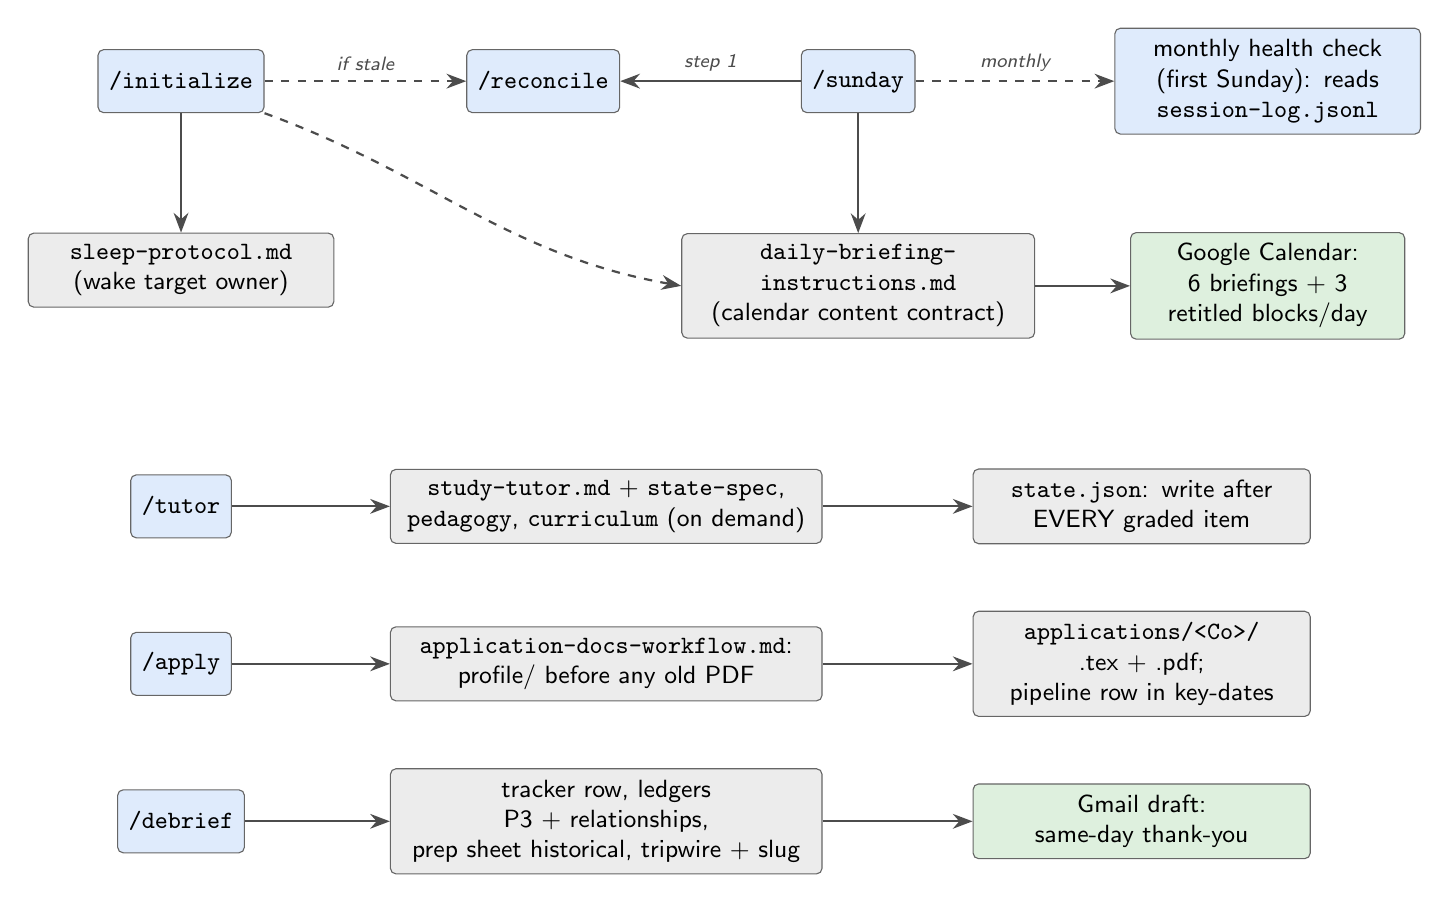
\begin{tikzpicture}
  \node[main] (init) at (0,0) {\texttt{/initialize}};
  \node[main] (recon) at (4.6,0) {\texttt{/reconcile}};
  \node[main] (sunday) at (8.6,0) {\texttt{/sunday}};
  \node[main, text width=36mm] (health) at (13.8,0) {monthly health check\\(first Sunday): reads\\\texttt{session-log.jsonl}};
  \node[file, text width=36mm] (sleep) at (0,-2.4) {\texttt{sleep-protocol.md}\\(wake target owner)};
  \node[file, text width=42mm] (dbi) at (8.6,-2.6) {\texttt{daily-briefing-}\\\texttt{instructions.md}\\(calendar content contract)};
  \node[ext, text width=32mm] (gcal2) at (13.8,-2.6) {Google Calendar:\\6 briefings + 3\\retitled blocks/day};

  \node[main] (tutor) at (0,-5.4) {\texttt{/tutor}};
  \node[file, text width=52mm] (st) at (5.4,-5.4) {\texttt{study-tutor.md} + \texttt{state-spec},\\\texttt{pedagogy}, \texttt{curriculum} (on demand)};
  \node[file, text width=40mm] (sjson) at (12.2,-5.4) {\texttt{state.json}: write after\\EVERY graded item};

  \node[main] (apply) at (0,-7.4) {\texttt{/apply}};
  \node[file, text width=52mm] (adw) at (5.4,-7.4) {\texttt{application-docs-workflow.md}:\\profile/ before any old PDF};
  \node[file, text width=40mm] (appout) at (12.2,-7.4) {\texttt{applications/<Co>/} .tex + .pdf;\\pipeline row in key-dates};

  \node[main] (debrief) at (0,-9.4) {\texttt{/debrief}};
  \node[file, text width=52mm] (dbout) at (5.4,-9.4) {tracker row, ledgers P3 + relationships,\\prep sheet historical, tripwire + slug};
  \node[ext, text width=40mm] (gmaild) at (12.2,-9.4) {Gmail draft:\\same-day thank-you};

  \draw[opt] (init) -- node[above, font=\scriptsize\itshape]{if stale} (recon);
  \draw[flow] (sunday) -- node[above, font=\scriptsize\itshape]{step 1} (recon);
  \draw[flow] (init) -- (sleep);
  \draw[flow] (sunday) -- (dbi);
  \draw[opt] (init.south east) to[out=-20,in=170] (dbi.west);
  \draw[flow] (dbi) -- (gcal2);
  \draw[opt] (sunday) -- node[above, font=\scriptsize\itshape]{monthly} (health);
  \draw[flow] (tutor) -- (st);
  \draw[flow] (st) -- (sjson);
  \draw[flow] (apply) -- (adw);
  \draw[flow] (adw) -- (appout);
  \draw[flow] (debrief) -- (dbout);
  \draw[flow] (dbout) -- (gmaild);
\end{tikzpicture}

\vspace{6mm}
{\large\bfseries 5. What the usage record shows (telemetry Jul 3--15, git Jun 9--Jul 15)}

\vspace{3mm}
\begin{tabular}{@{}llll@{}}
\toprule
Workflow & Logged uses & Subagents observed & Note \\
\midrule
\texttt{/reconcile} & 5 & yes (3 of 5, post Jul-8 upgrade) & near-daily in W28, then 4 dark days \\
system (audit/upgrade) & 2 & varies & Jul 3 migration, Jul 8 upgrade \\
\texttt{/sunday} & 1 & via nested reconcile & Jul 12 Sunday MISSED (1 of 2 hit) \\
\texttt{/debrief} & 1 & none & Anicito, loop closed latency 0 \\
quick / ad-hoc & 1 & none & a backfilled reconstruction line \\
\texttt{/tutor} & 0 logged & none & 4 sessions exist in state.json, pre-telemetry \\
\texttt{/apply} & 0 logged & none & 15 application folders predate telemetry \\
\texttt{/initialize} & 0 (not in schema enum) & --- & schema gap, audit item Q3 \\
\bottomrule
\end{tabular}

\vspace{4mm}
Cadence: 10 sessions over 13 days, 5 days dark (38\%); 187 commits in 37 days, batch-committed at session end. Highest-yield drift sensor in practice: Veer's own screenshots (3 of the last 4 reconciles), covering exactly the channels the scans cannot read (iMessage, WhatsApp). Full findings and the ranked improvement list: \texttt{specs/2026-07-15-system-audit.md}.

\end{document}
